\section{Data Storage}
  \subsection{Session}
    Session that used to determine which user is currently posting request is stored in redis which is a light key-value pair database.
    Though only one value can be stored in one key, its high performance makes it's the best to store sessions data.

    The sessions is stored automatically without any design, for a third party package will handle all of this.

  \subsection{Item}
    Item mainly is the only things that we need to store other than user's information which needed for all apps.

    With considering of that each piece of information mainly doesn't have relationship with others but has multiple complex attributes in itself,
    NoSQL that doesn't need table structure but store data in documents is what we want.

    An item will be mapped into a FetcherContext object in program, and it will be stored into database simply with all attributes
    in key-value pair format.

    \begin{figure}[H]
      \centering
      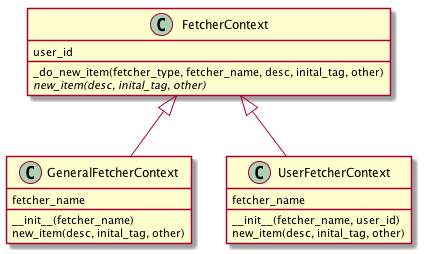
\includegraphics[width=0.6\textwidth]{img/fetcherContext.png}
      \caption{FetcherContext\label{fig:fetcherContext}}
    \end{figure}

  \subsection{Labels}
    Labels is a quite simple one in storage step.
    Each label is just a basic string describing itself. So it doesn't have even an individual table.
    Labels are stored as a part of Item, in a list as a sub node of it.

    For performance reason, Labels are often used to filtering out Items, so index was build according to it.

